\documentclass[11pt,dvipdfmx,a4paper]{jsarticle}

\usepackage{amsmath,amssymb}
\usepackage{bm}
\usepackage[dvipdfmx]{graphicx}
\usepackage{physics} % http://mirrors.ibiblio.org/CTAN/macros/latex/contrib/physics/physics.pdf
\usepackage{siunitx} %SI単位を楽に出力
\usepackage{mathtools} %環境の追加
% \usepackage{circuitikz} %電気回路をtex中で書く
% \usepackage{caption} %番号なしキャプションを書く
% \usepackage{cancel} %式中に斜線を入れる
% \usepackage{tensor} %テンソルの添え字を書く
% \usepackage{tikz} %図を書く
% \usepackage{ascmac} %四角い枠の中に文章を書く
% \usepackage{float} %figureで[hbp]オプションを使う
% \usepackage{hyperref}  \usepackage{pxjahyper} %ハイパーリンクをつかう
% \usepackage{tablefootnote} %表中に注釈をいれる
% \usepackage[thicklines]{cancel} %数式中の取り消し線
% \usepackage[version=4]{mhchem} %化学式の入力
\usepackage{pdfpages}
% \usepackage{wrapfig} %文章の回り込み
\usepackage[subrefformat=parens]{subcaption} %(a)図のようにすることができるやつ
\usepackage{here}
\usepackage[margin=15mm]{geometry} %余白の削除

\graphicspath{{./image/}}

\begin{document}

%出力したpdfを表紙にするとき
% \includepdf[pages=1,noautoscale=false]{cover.pdf}
% \newpage

%texで表紙を書くとき
\quad\\[35mm]
\centerline{\Huge{\textsf{第 1 回}}}
\quad\\[5mm]
\centerline{\Huge{\textsf{応 用 物 理 学 実 験}}}
\quad\\[5mm]
\begin{table}[h]
	\centering
	\begin{tabular}{| c | c |}
		\hline
		\Huge\textsf{{題目}} & \Huge{\textsf{X 線回折}} \rule[-5mm]{0mm}{15mm} \\
		\hline
	\end{tabular}
\end{table}
\quad\\[10mm]
\begin{table}[h]
	\centering
	\begin{tabular}{l l}
		\hline
		\LARGE{\textsf{氏\qquad 名}} & \LARGE{\textsf{: 西原 翔}} \rule[0mm]{0mm}{6mm} \\
		\hline
		\LARGE{\textsf{学  籍  番  号}} & \LARGE{\textsf{: 1522068}} \rule[0mm]{0mm}{6mm} \\
		\LARGE{\textsf{学部学科学年}} & \LARGE{\textsf{: 理学部第一部応用物理学科3年}}\\
		\hline
	\end{tabular}
\end{table}
\quad\\[10mm]
\centerline{\LARGE{\textsf{共同実験者:1522064 中井空弥}}}\\[2mm]
\centerline{\LARGE{\textsf{\qquad\qquad\quad\;\;1522091 宮田祟杜}}}\\[2mm]
\centerline{\LARGE{\textsf{\qquad\qquad\quad\;\;1522095 村山涼矢}}}\\[2mm]
\centerline{\LARGE{\textsf{\qquad\qquad\quad\;\;1522B02 中村洸太}}}\\[2mm]
\quad\\[10mm]
\centerline{\LARGE{\textsf{提出年月日:2024年05月02日}}}\\[2mm]
\centerline{\LARGE{\textsf{実験実施日:2024年04月19日}}}\\[2mm]
\centerline{\LARGE{\textsf{\qquad\qquad\quad\;2024年04月26日}}}
\quad\\[10mm]
\centerline{\LARGE{\textsf{東 京 理 科 大 学 理 学 部 第 1 部}}}\\[2mm]
\centerline{\LARGE{\textsf{応 用 物 理 学 教 室}}}

\thispagestyle{empty}
\clearpage
\addtocounter{page}{-1}
\newpage

% \twocolumn
\section{目的}
粉末試料に X 線を入射したときの回折パターンから、その試料の結晶構造を推定する。
% もうちょい書きたい

\section{原理}
\subsection{回折の一般論}
\subsection{ラウエの回折条件}
% Ewalt 球らへんでアンブレラ効果をやりたい
\subsection{ブラッグの回折条件}
\subsection{結晶構造因子}
\subsection{X 線源}
今回の実験で使う X 線源はタングステンフィラメントを加熱し発生した熱電子を加速しCuにあてて、
光電効果により発生させる。
この際、銅原子内の電子が様々な準位に励起され、励起により空いた準位に電子が遷移する際に光子(X 線)を放つ。
特に
2p 軌道から励起より空いた 1s 軌道に遷移するとき発生する X 線は K\(\alpha\) 線、
3p 軌道から励起より空いた 1s 軌道に遷移するとき発生する X 線は K\(\alpha\) 線と呼ばれる。
さらに微細構造によりK\(\alpha\)は二つに分裂しておりそれぞれを
K\(\alpha_1\) 線、K\(\alpha_2\) 線と呼ばれる。

K\(\alpha_1\) 線、K\(\alpha_2\) 線K、K\(\beta\) 線の波長はそれぞれ
\begin{align}
	\lambda_{\alpha1} = 1.542 \text{\AA}\\
	\lambda_{\alpha2} = 1.540 \text{\AA}\\
	\lambda_{\alpha1} = 1.392 \text{\AA}\\
\end{align}
というように近い値をもつ。\cite{rikanenpyo}
これらは無視できない強度を持ち X 線の回折パターンに影響与えるためうまく取り除く必要がある。

Ni の 1s 軌道電子が空軌道へ遷移するのに必要なエネルギーの最低値が 8332.8 eV であるつまり、
Ni が吸収する波長のうち最も長いものは \(\lambda = 1.488\) \AA である。
これを利用して X 線のディテクターの前に Ni のフィルターをセットすることで K\(\beta\) 線のピークをなくすことができる。

K\(\alpha_2\) 線は波長が近いためこれによるピークが見えるものと見えないものがある。
これは測定装置に付属する解析ソフトにより除去する。


\section{実験}
この実験ではリガクの MiniFlex600 を用いて、
Cu, Si, Fe の単体粉末と、NaCl, KCl, CsCl の粉末の X 線回折パターンを測定した。
その際、Ni フィルターによる K\(\beta\)線 の除去の程度を調べるため、
Cu の X 線の回折パターンはフィルターが無いときとある時の両方を測定した。
測定データはピークの位置や回折強度に大きな影響を与えない程度のバックグラウンド除去や
K\(\alpha_2\) 線によるピークを除去をした。

\section{結果}
Niフィルターの有無による Cu の X 線回折パターンは図\ref{Cu_XRD}のようになった。
Si, Fe の単体粉末と、NaCl, KCl, CsCl の粉末の X 線回折パターンは
それぞれ図\ref{Si_XRD}, 図\ref{Fe_XRD}, 図\ref{NaCl_XRD}, 図\ref{KCl_XRD}, 図\ref{CsCl_XRD} のようになった。
% \begin{figure}[h]
% 	\centering
% 	\begin{minipage}[t]{0.48\columnwidth}
% 		\centering
% 		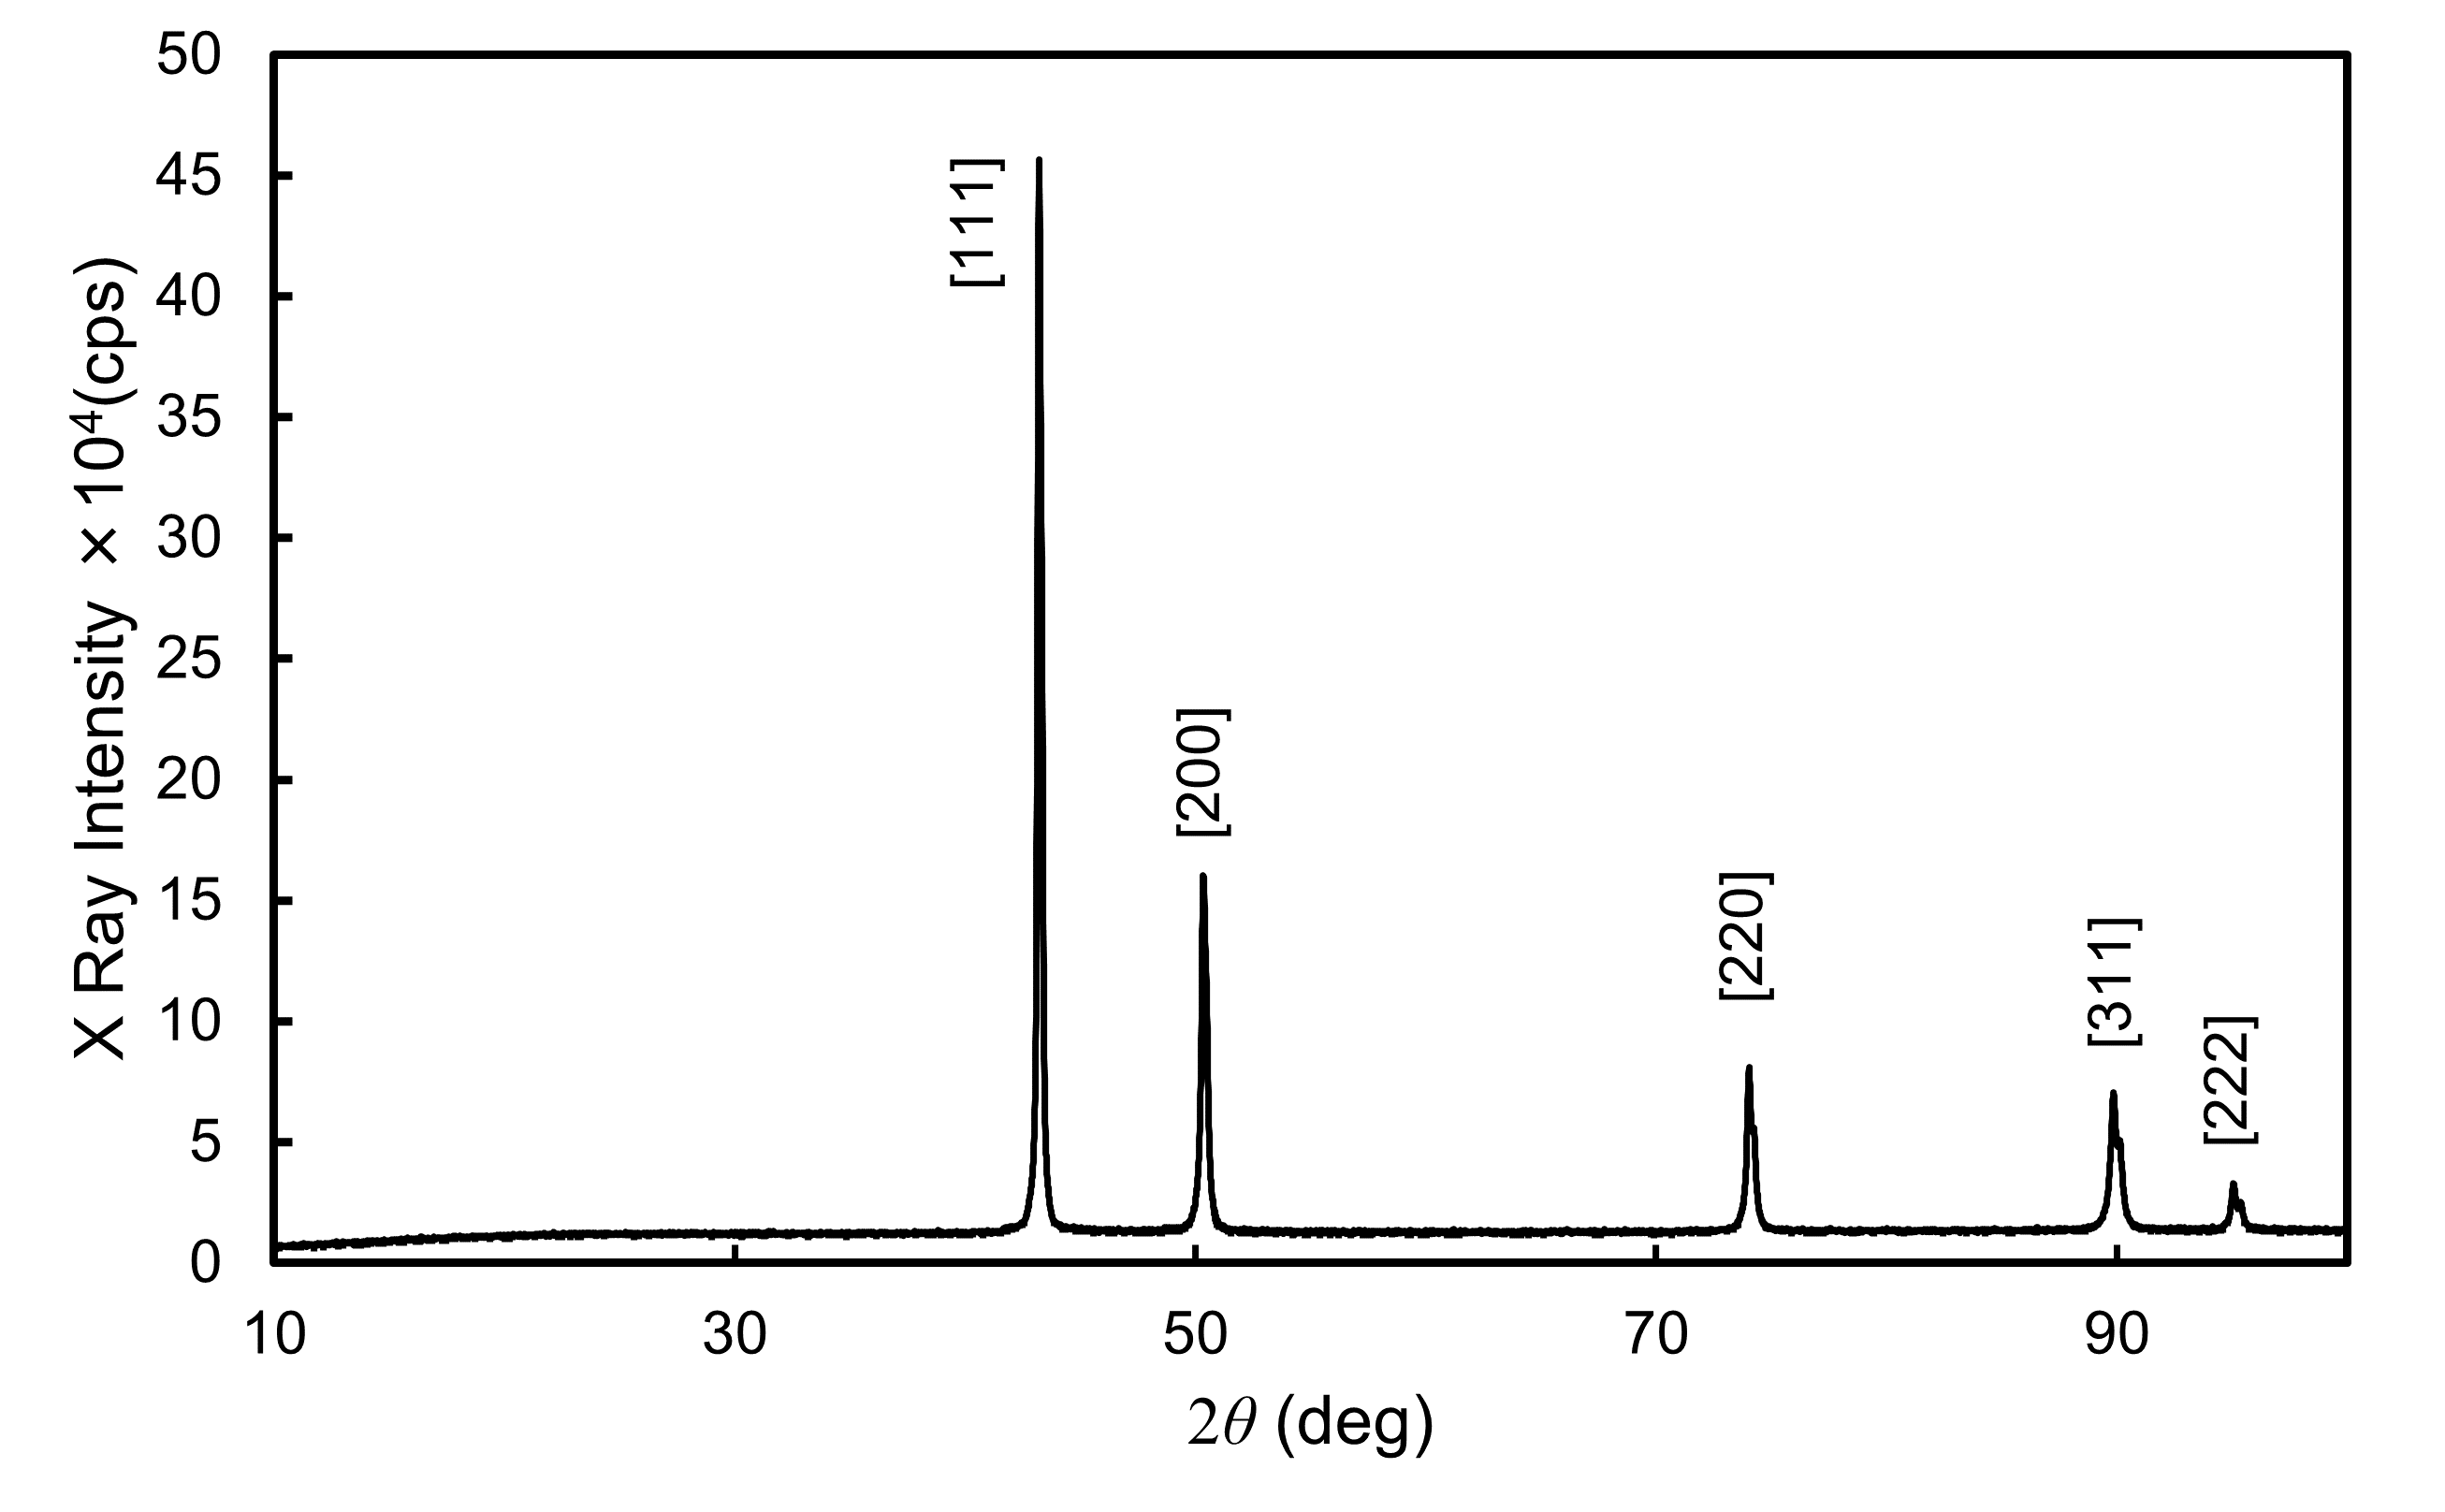
\includegraphics[width=\columnwidth]{/graph/Cu.png}
% 		\subcaption{Ni フィルター有}
% 	\end{minipage}
% 	\hfil
% 	\begin{minipage}[t]{0.48\columnwidth}
% 		\centering
% 		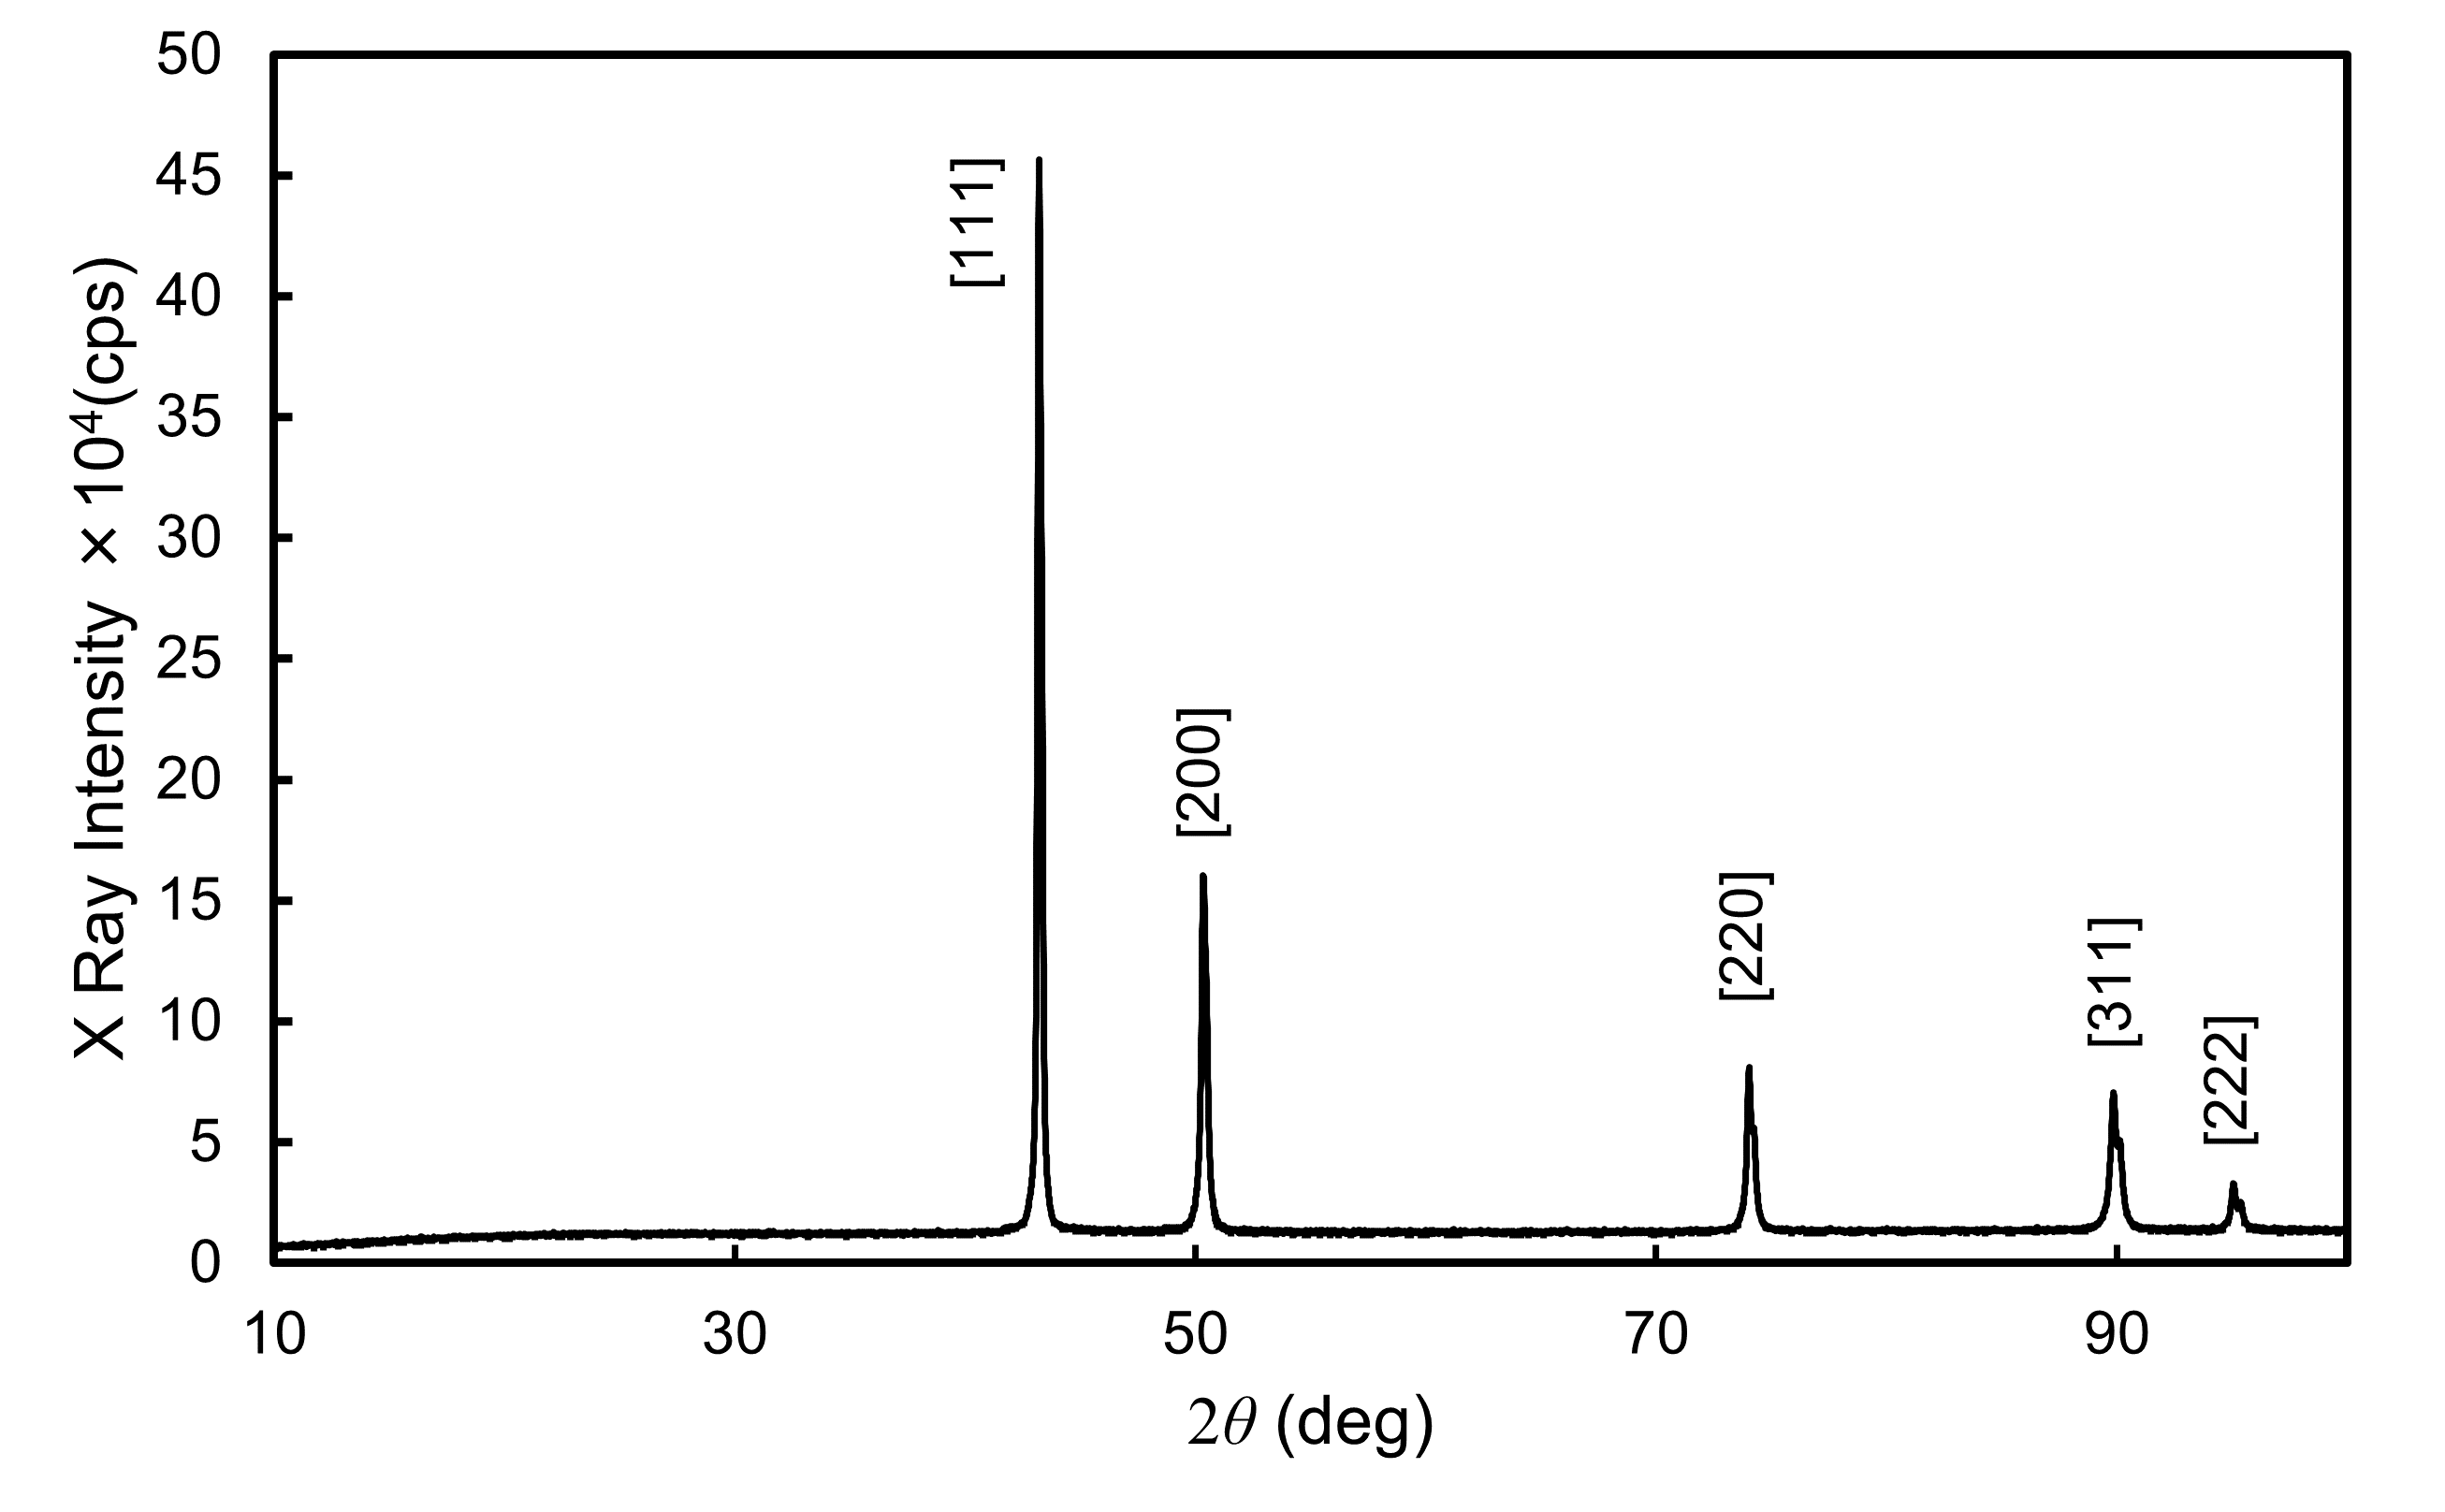
\includegraphics[width=\columnwidth]{/graph/Cu.png}
% 		\subcaption{Ni フィルター無}
% 	\end{minipage}
% 	\caption{Cu 単体粉末の X 線回折強度}
% 	\label{Cu_XRD}
% \end{figure}
% \begin{figure}[h]
% 	\centering
% 	\begin{minipage}[t]{0.48\columnwidth}
% 		\centering
% 		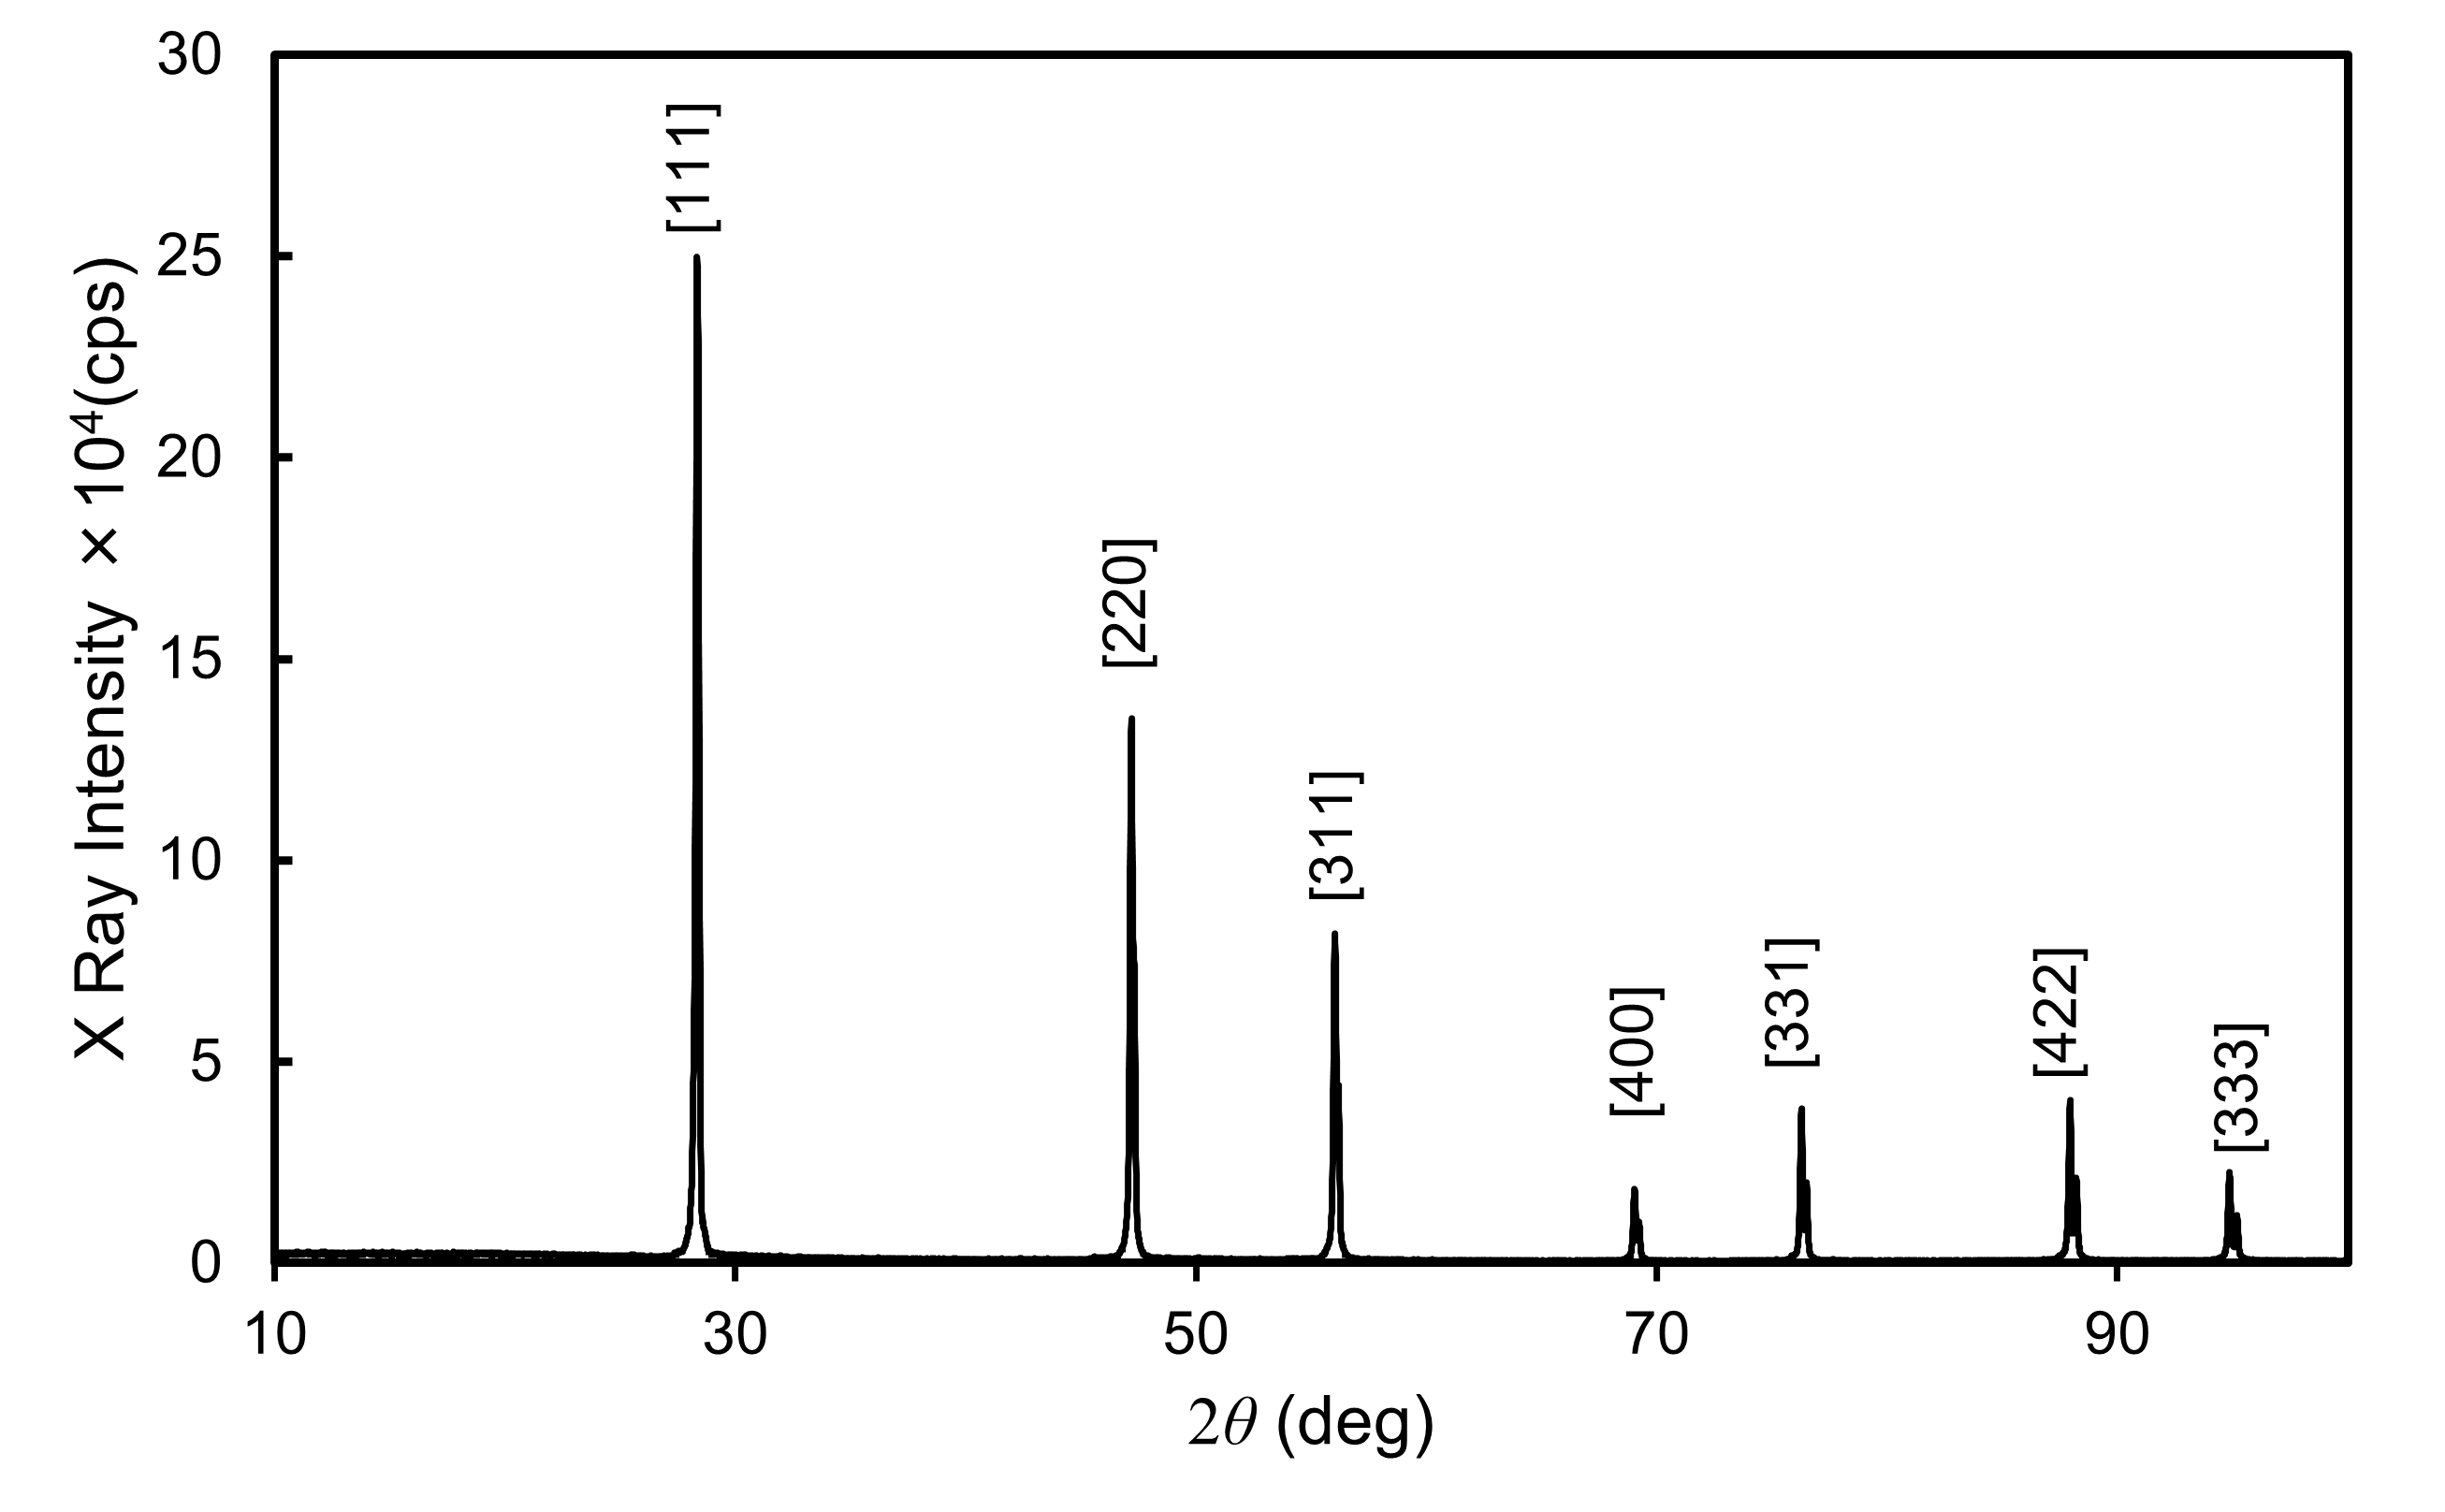
\includegraphics[width=\columnwidth]{/graph/Si.png}
% 		\caption{Si 単体粉末の X 線回折強度}
% 		\label{Si_XRD}
% 	\end{minipage}
% 	\hfil
% 	\begin{minipage}[t]{0.48\columnwidth}
% 		\centering
% 		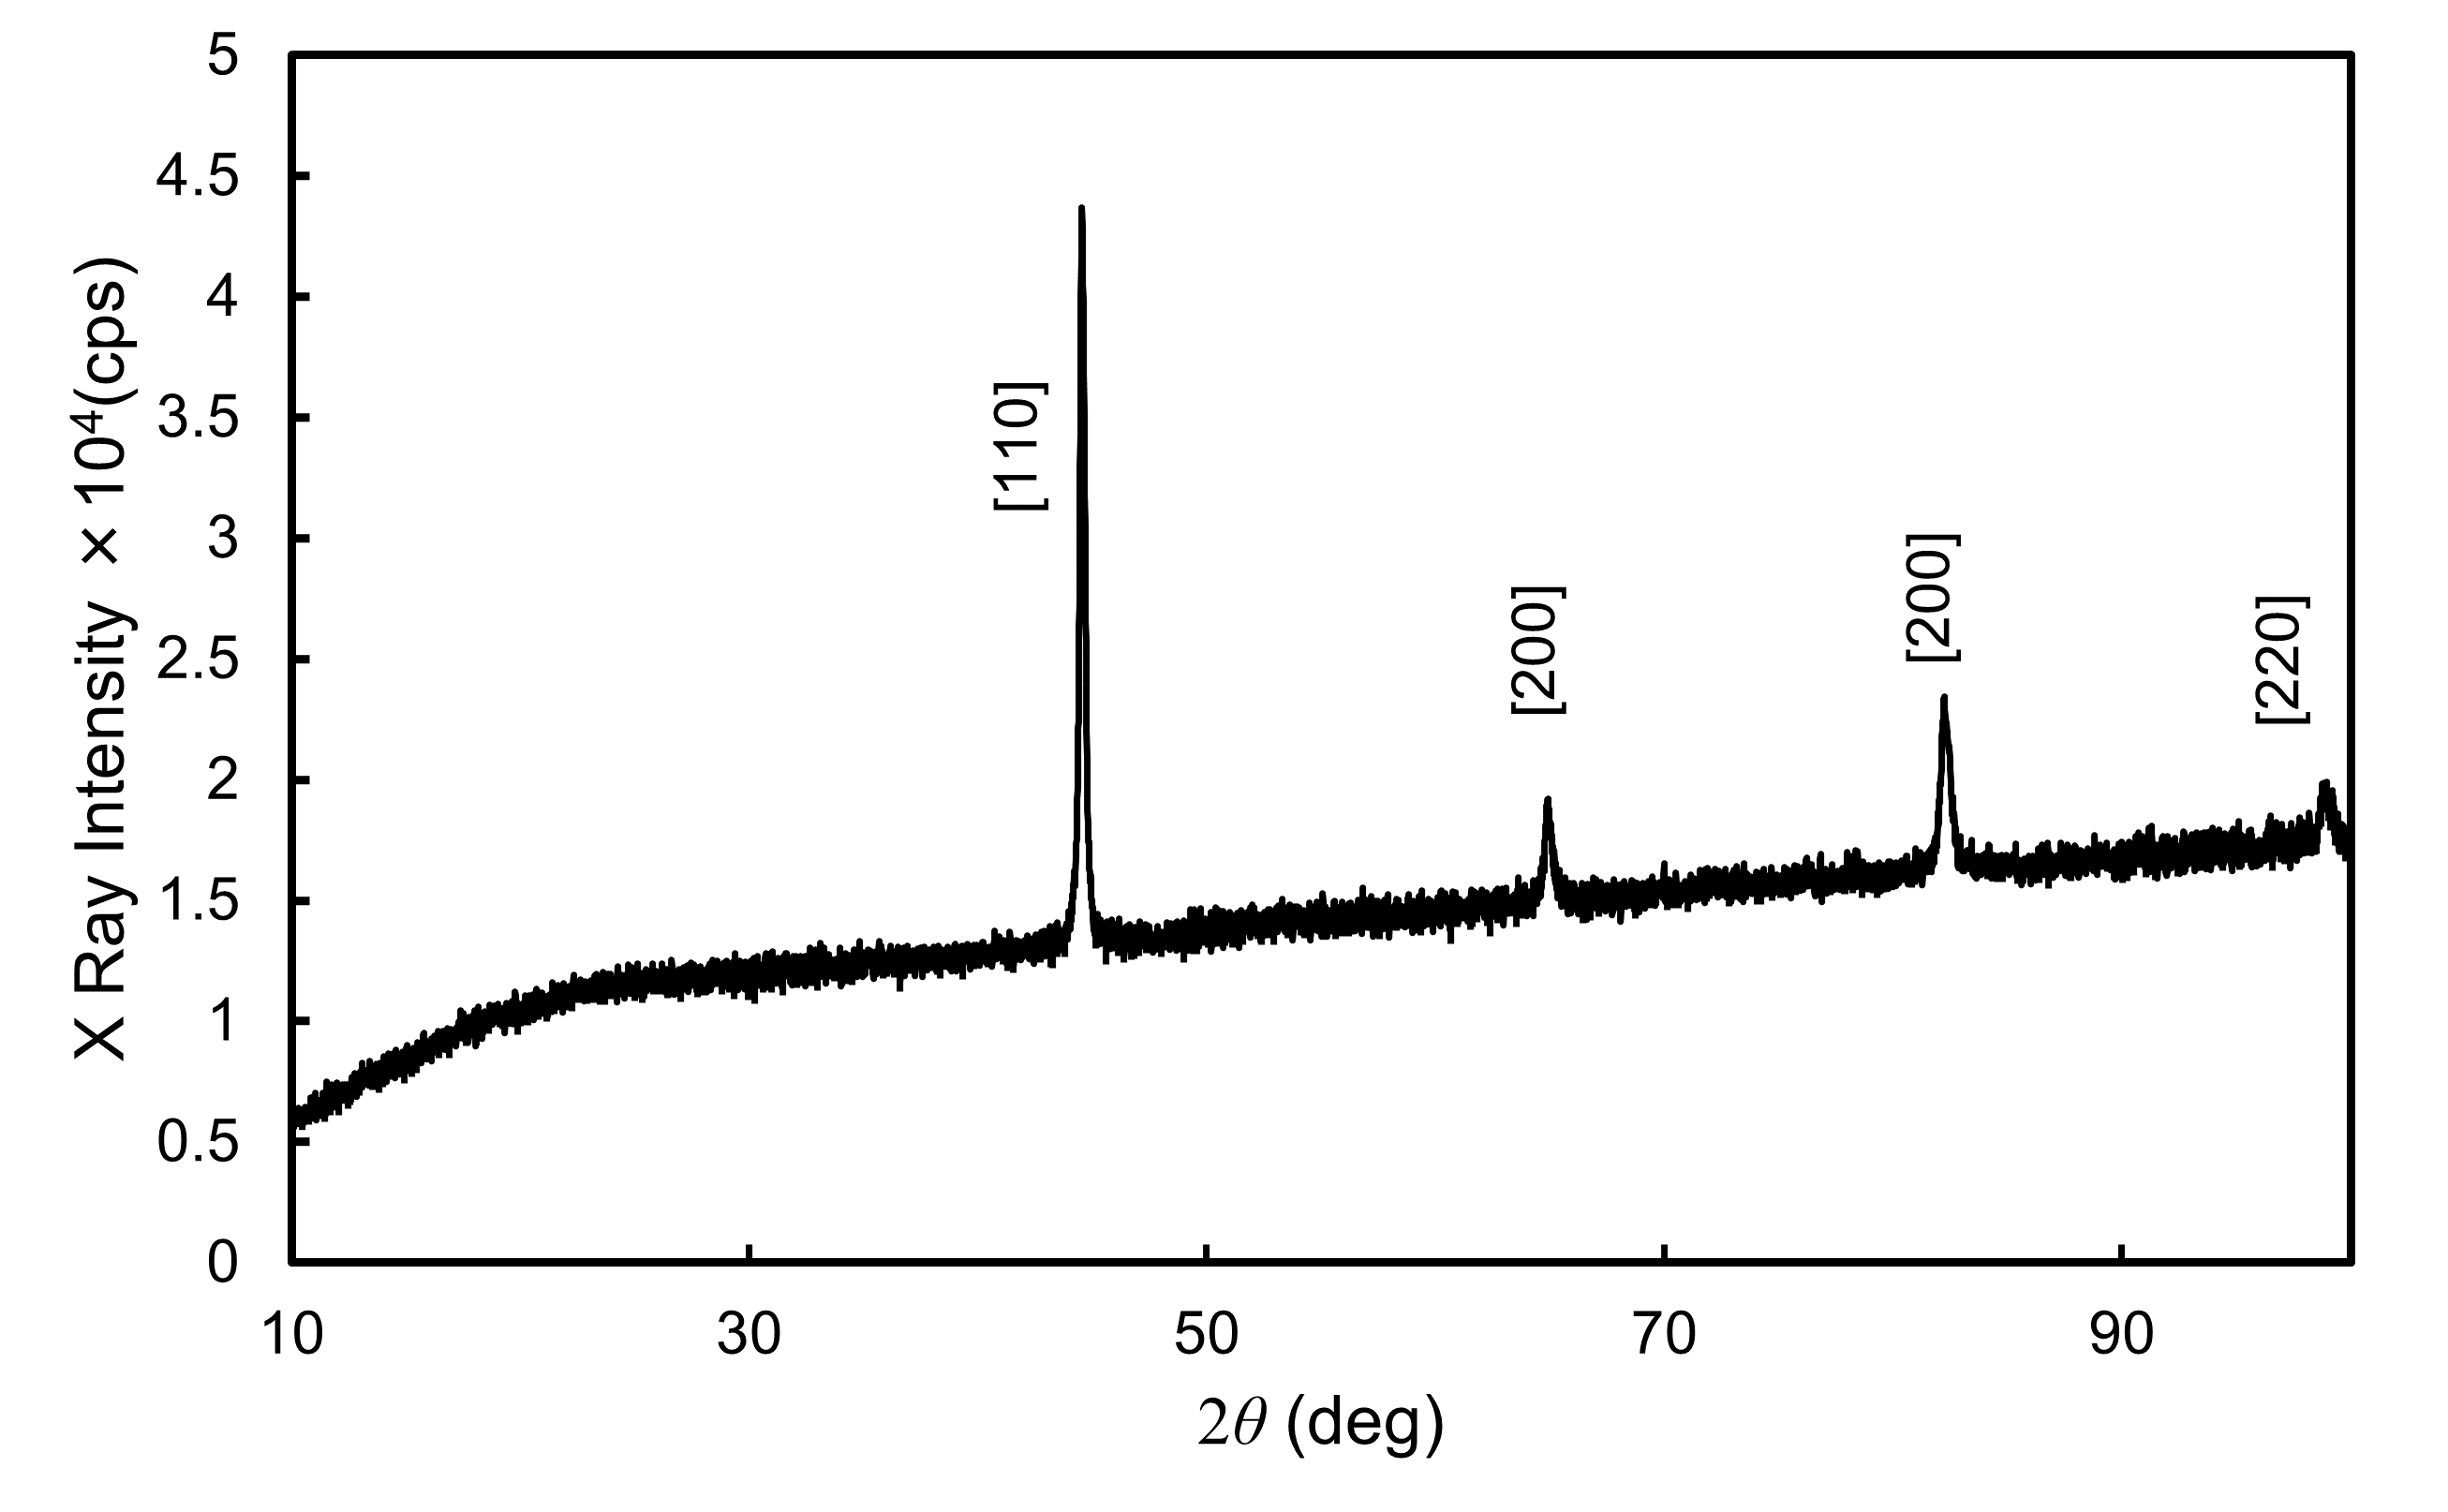
\includegraphics[width=\columnwidth]{/graph/Fe.png}
% 		\caption{Fe 単体粉末の X 線回折強度}
% 		\label{Fe_XRD}
% 	\end{minipage}
% \end{figure}
% \begin{figure}[h]
% 	\centering
% 	\begin{minipage}[t]{0.48\columnwidth}
% 		\centering
% 		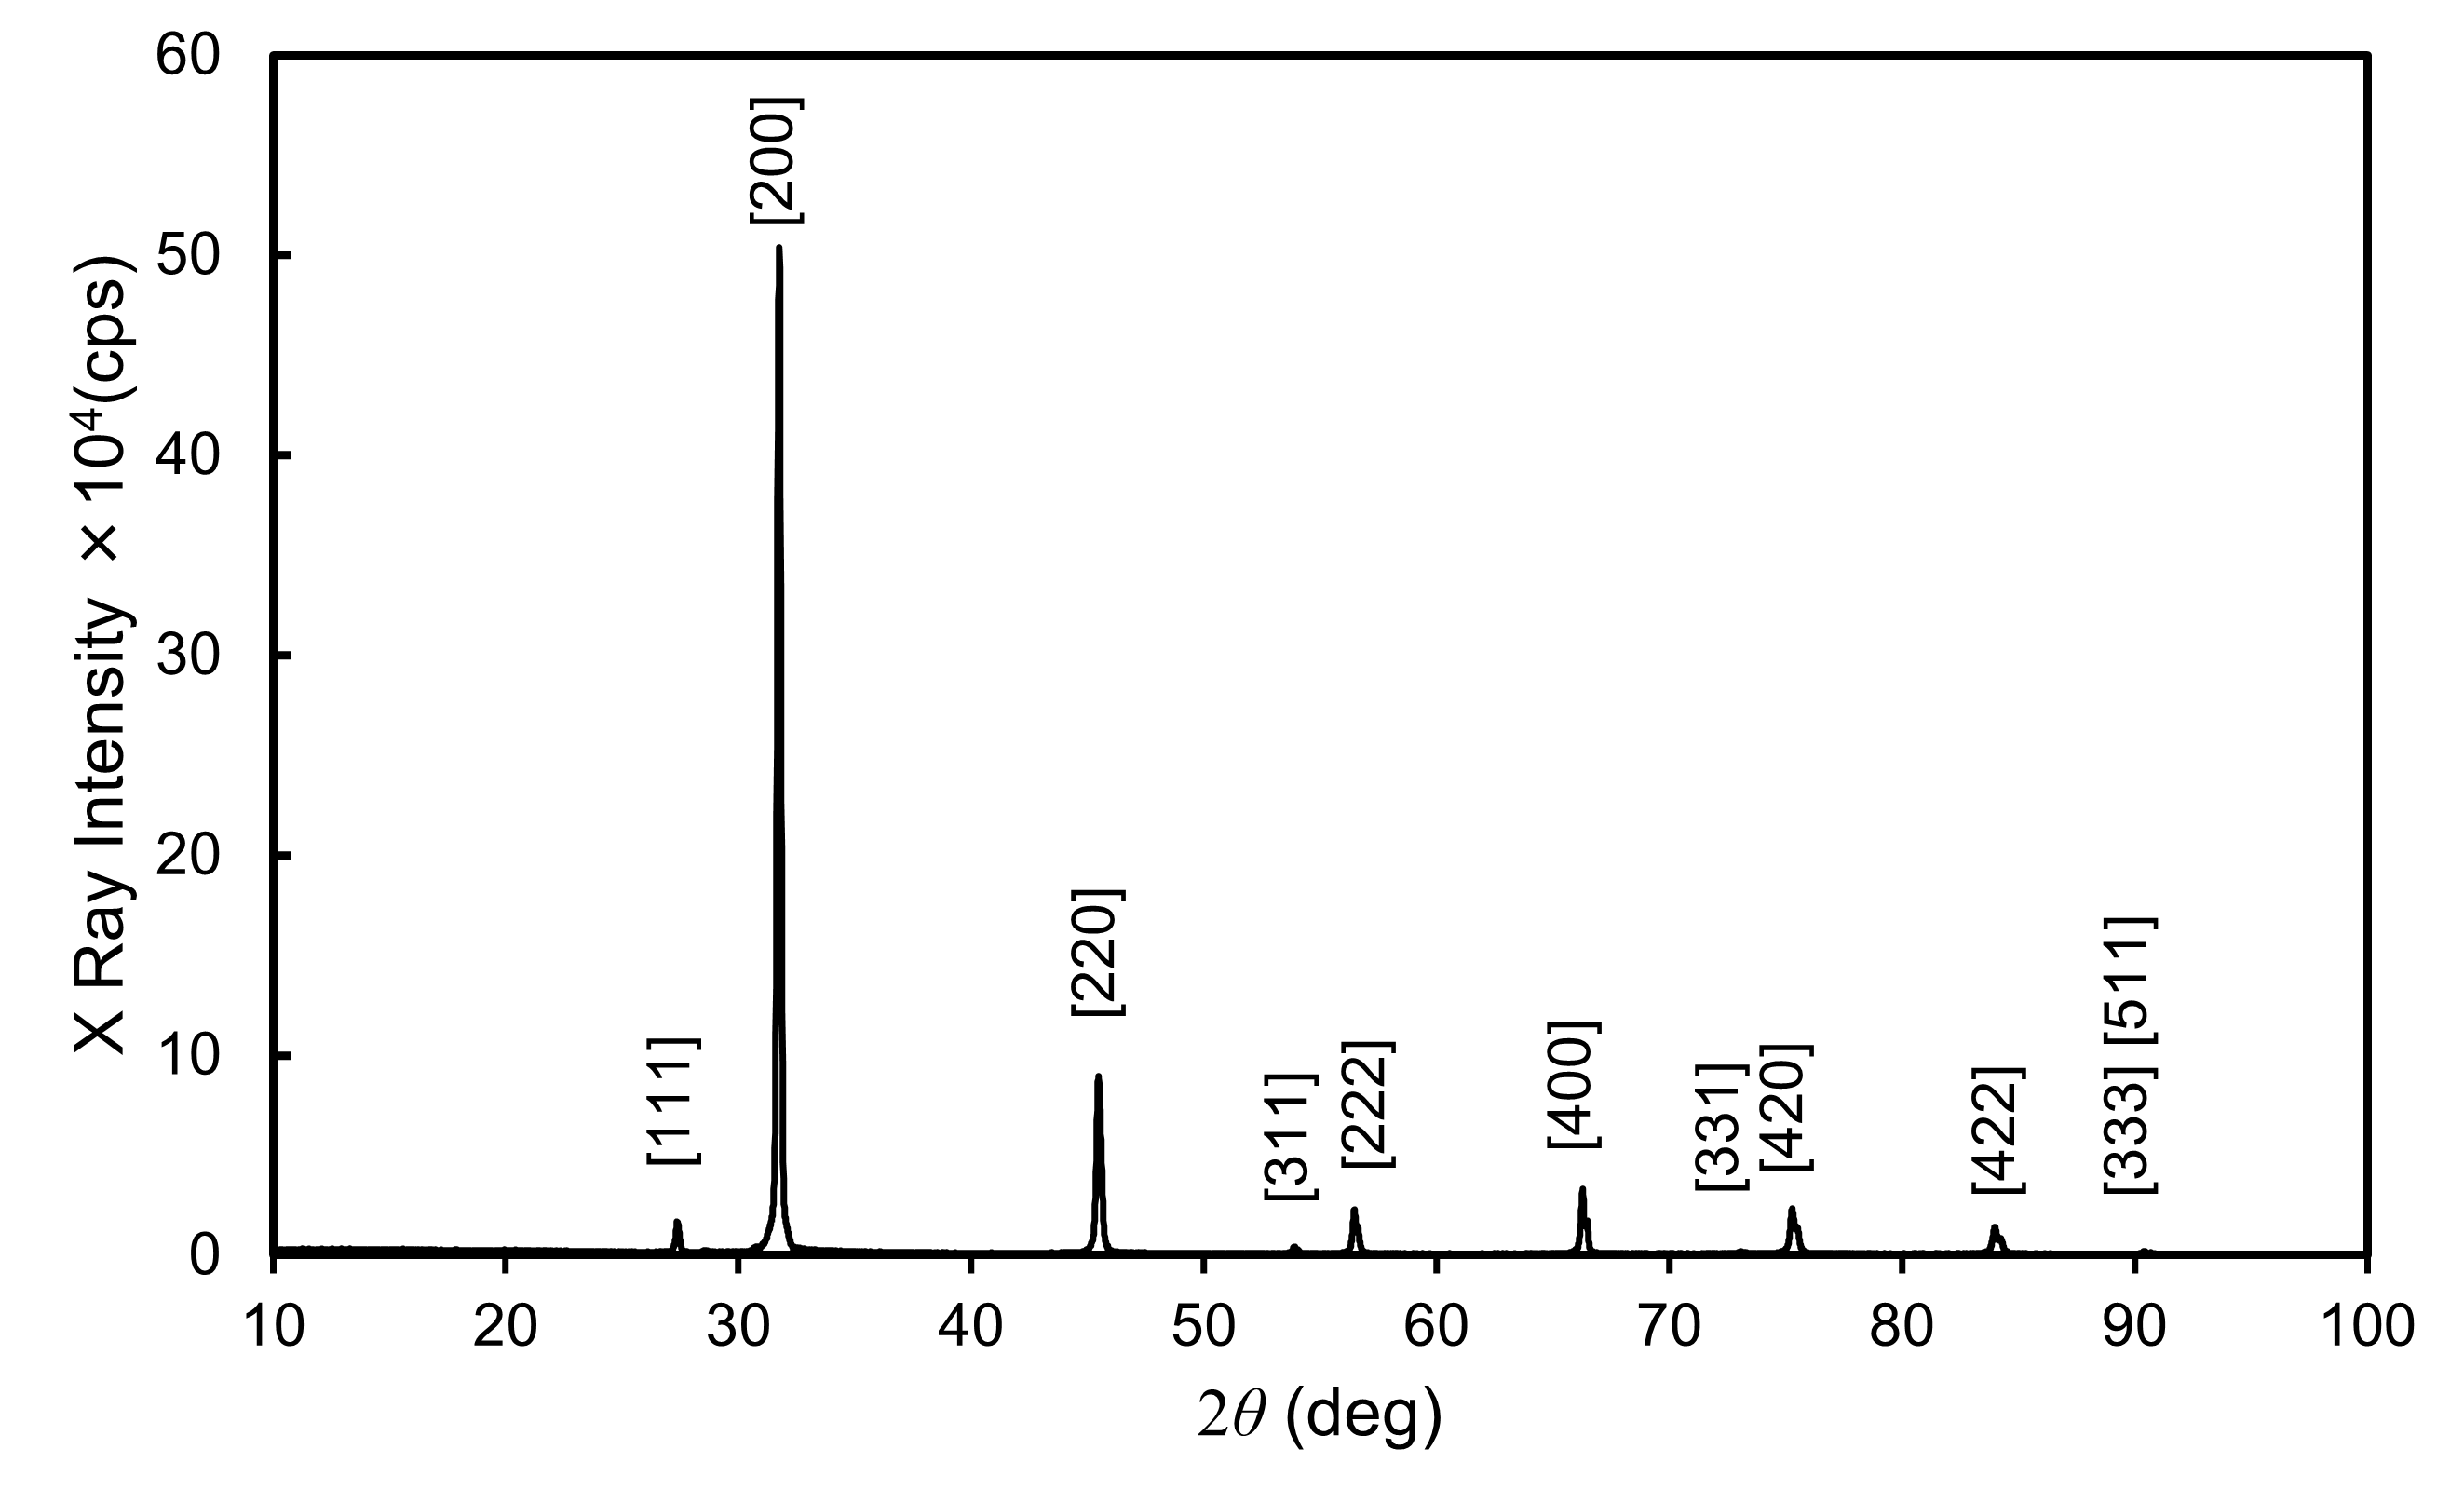
\includegraphics[width=\columnwidth]{/graph/NaCl.png}
% 		\caption{NaCl 粉末の X 線回折強度}
% 		\label{NaCl_XRD}
% 	\end{minipage}
% 	\hfil
% 	\begin{minipage}[t]{0.48\columnwidth}
% 		\centering
% 		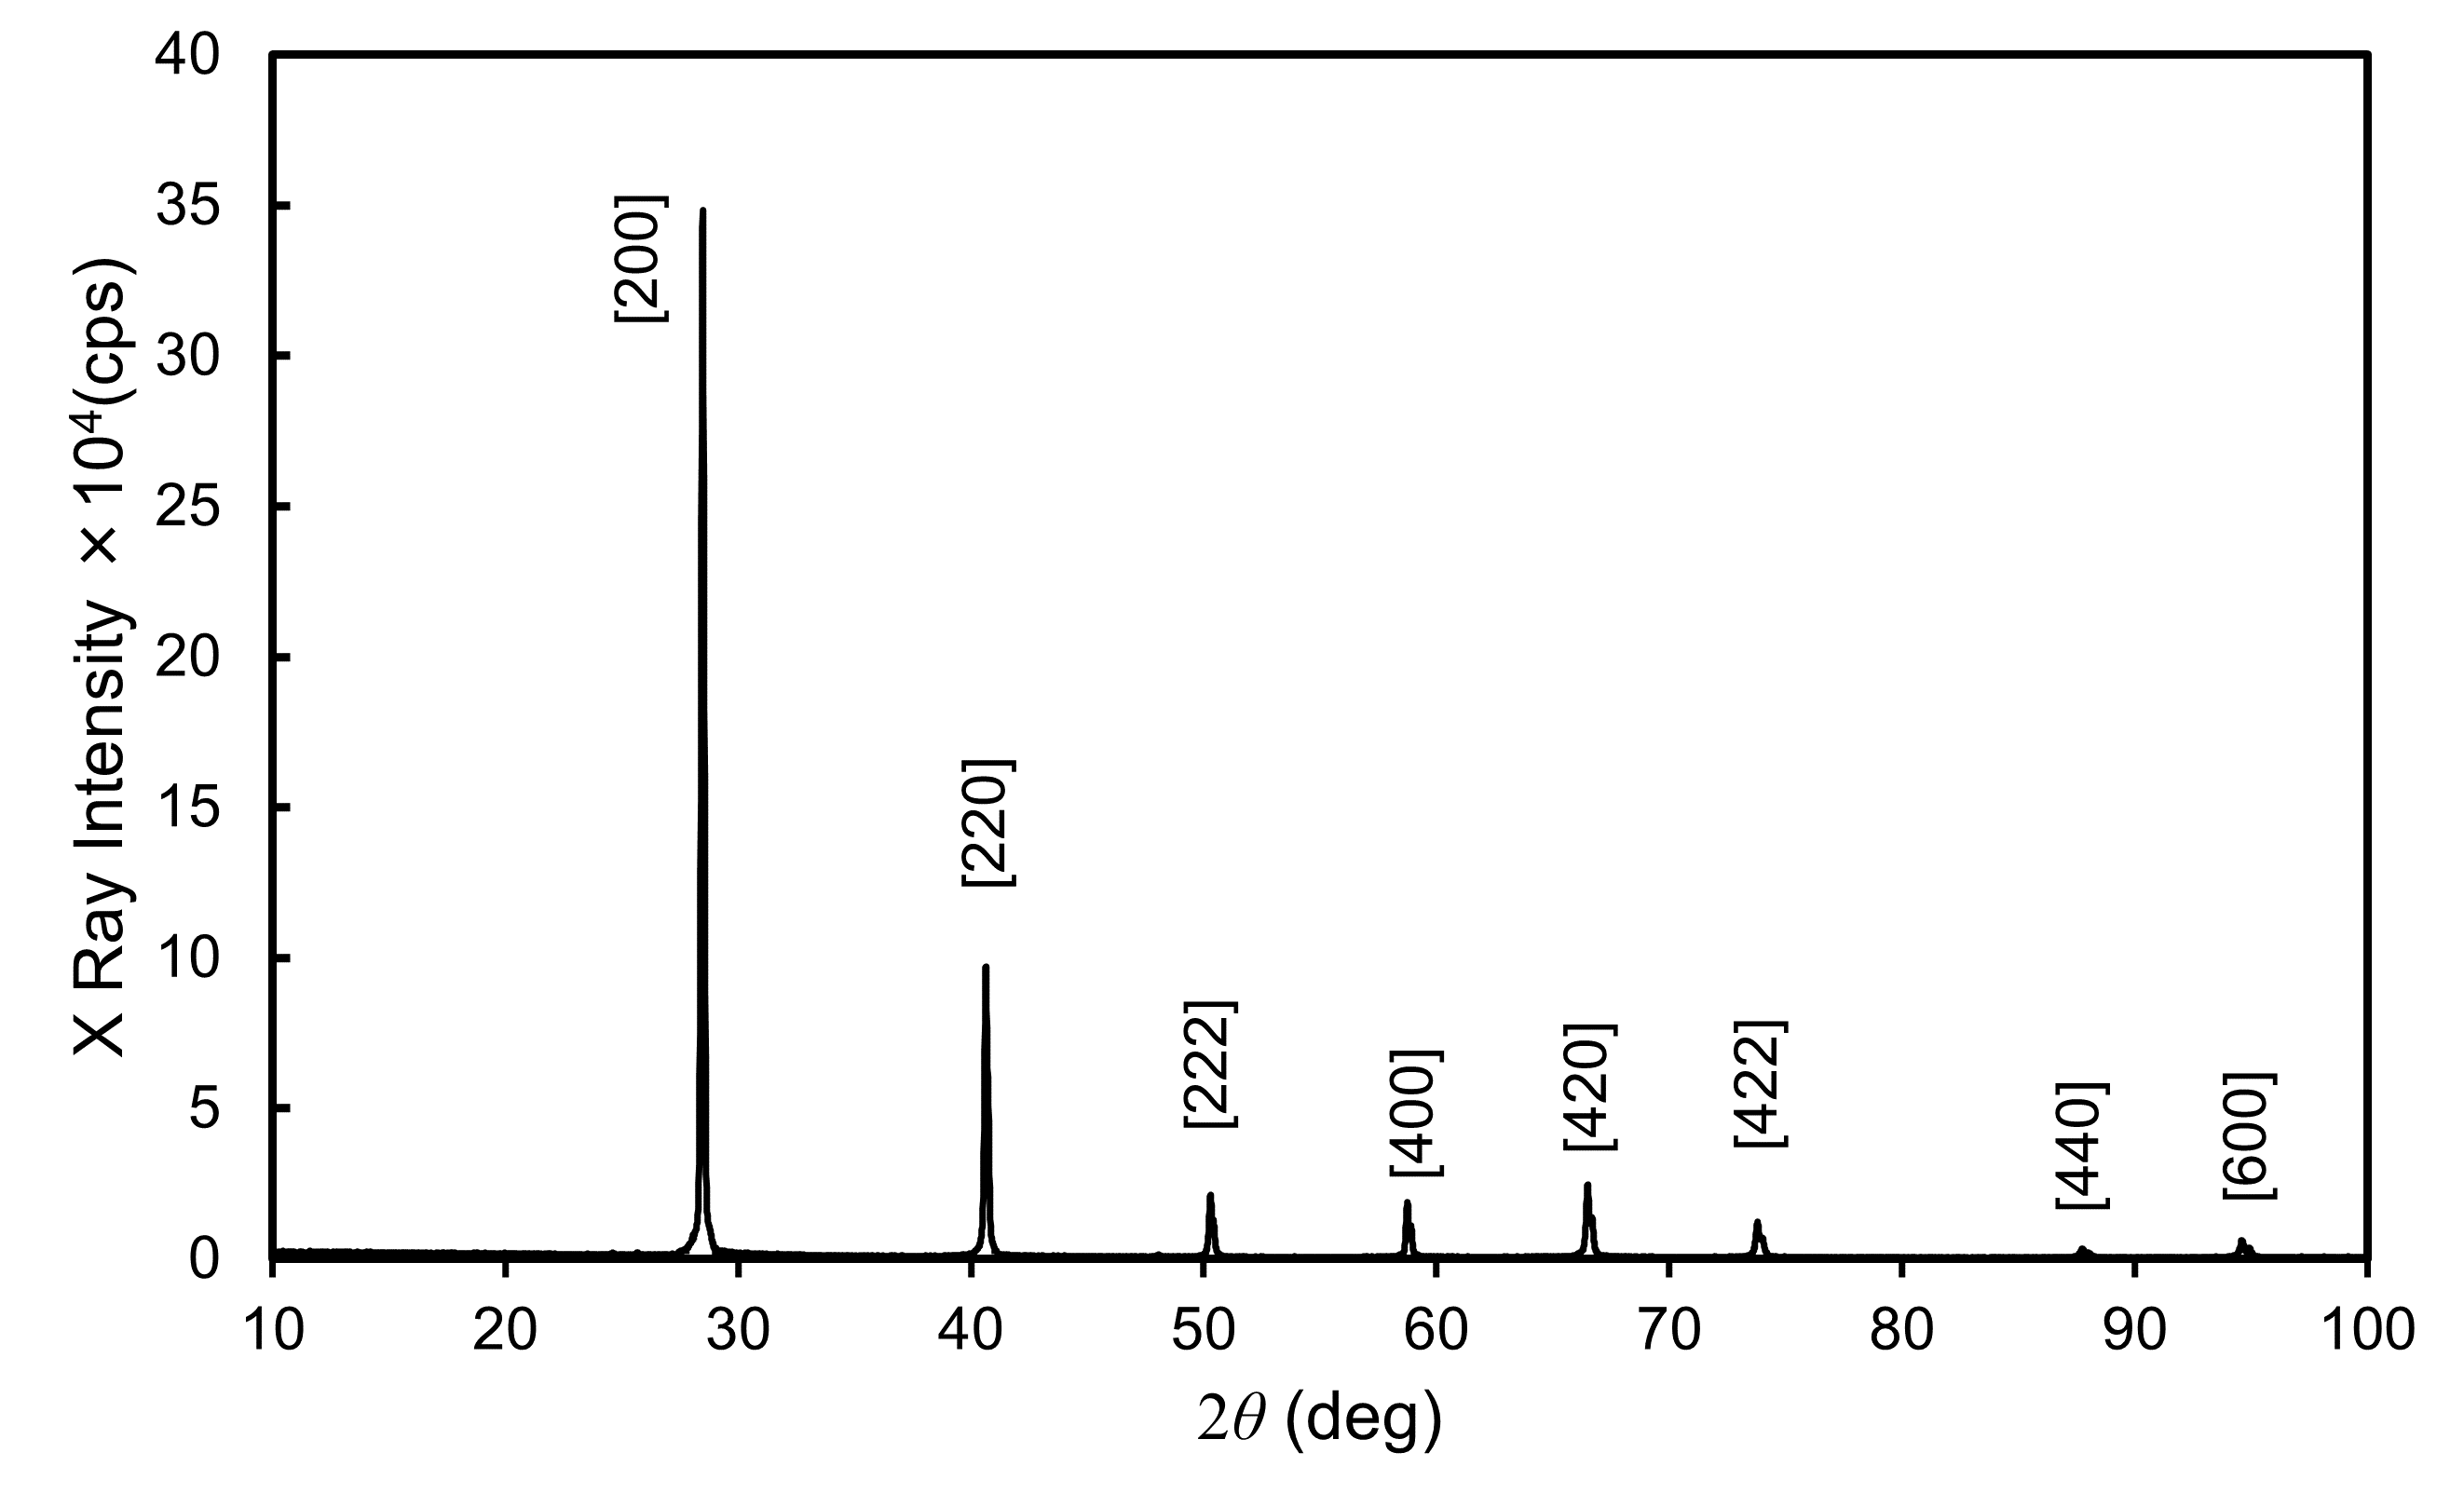
\includegraphics[width=\columnwidth]{/graph/KCl.png}
% 		\caption{KCl 粉末の X 線回折強度}
% 		\label{KCl_XRD}
% 	\end{minipage}
% \end{figure}
% \begin{figure}[h]
% 	\centering
% 	\begin{minipage}[t]{0.48\columnwidth}
% 		\centering
% 		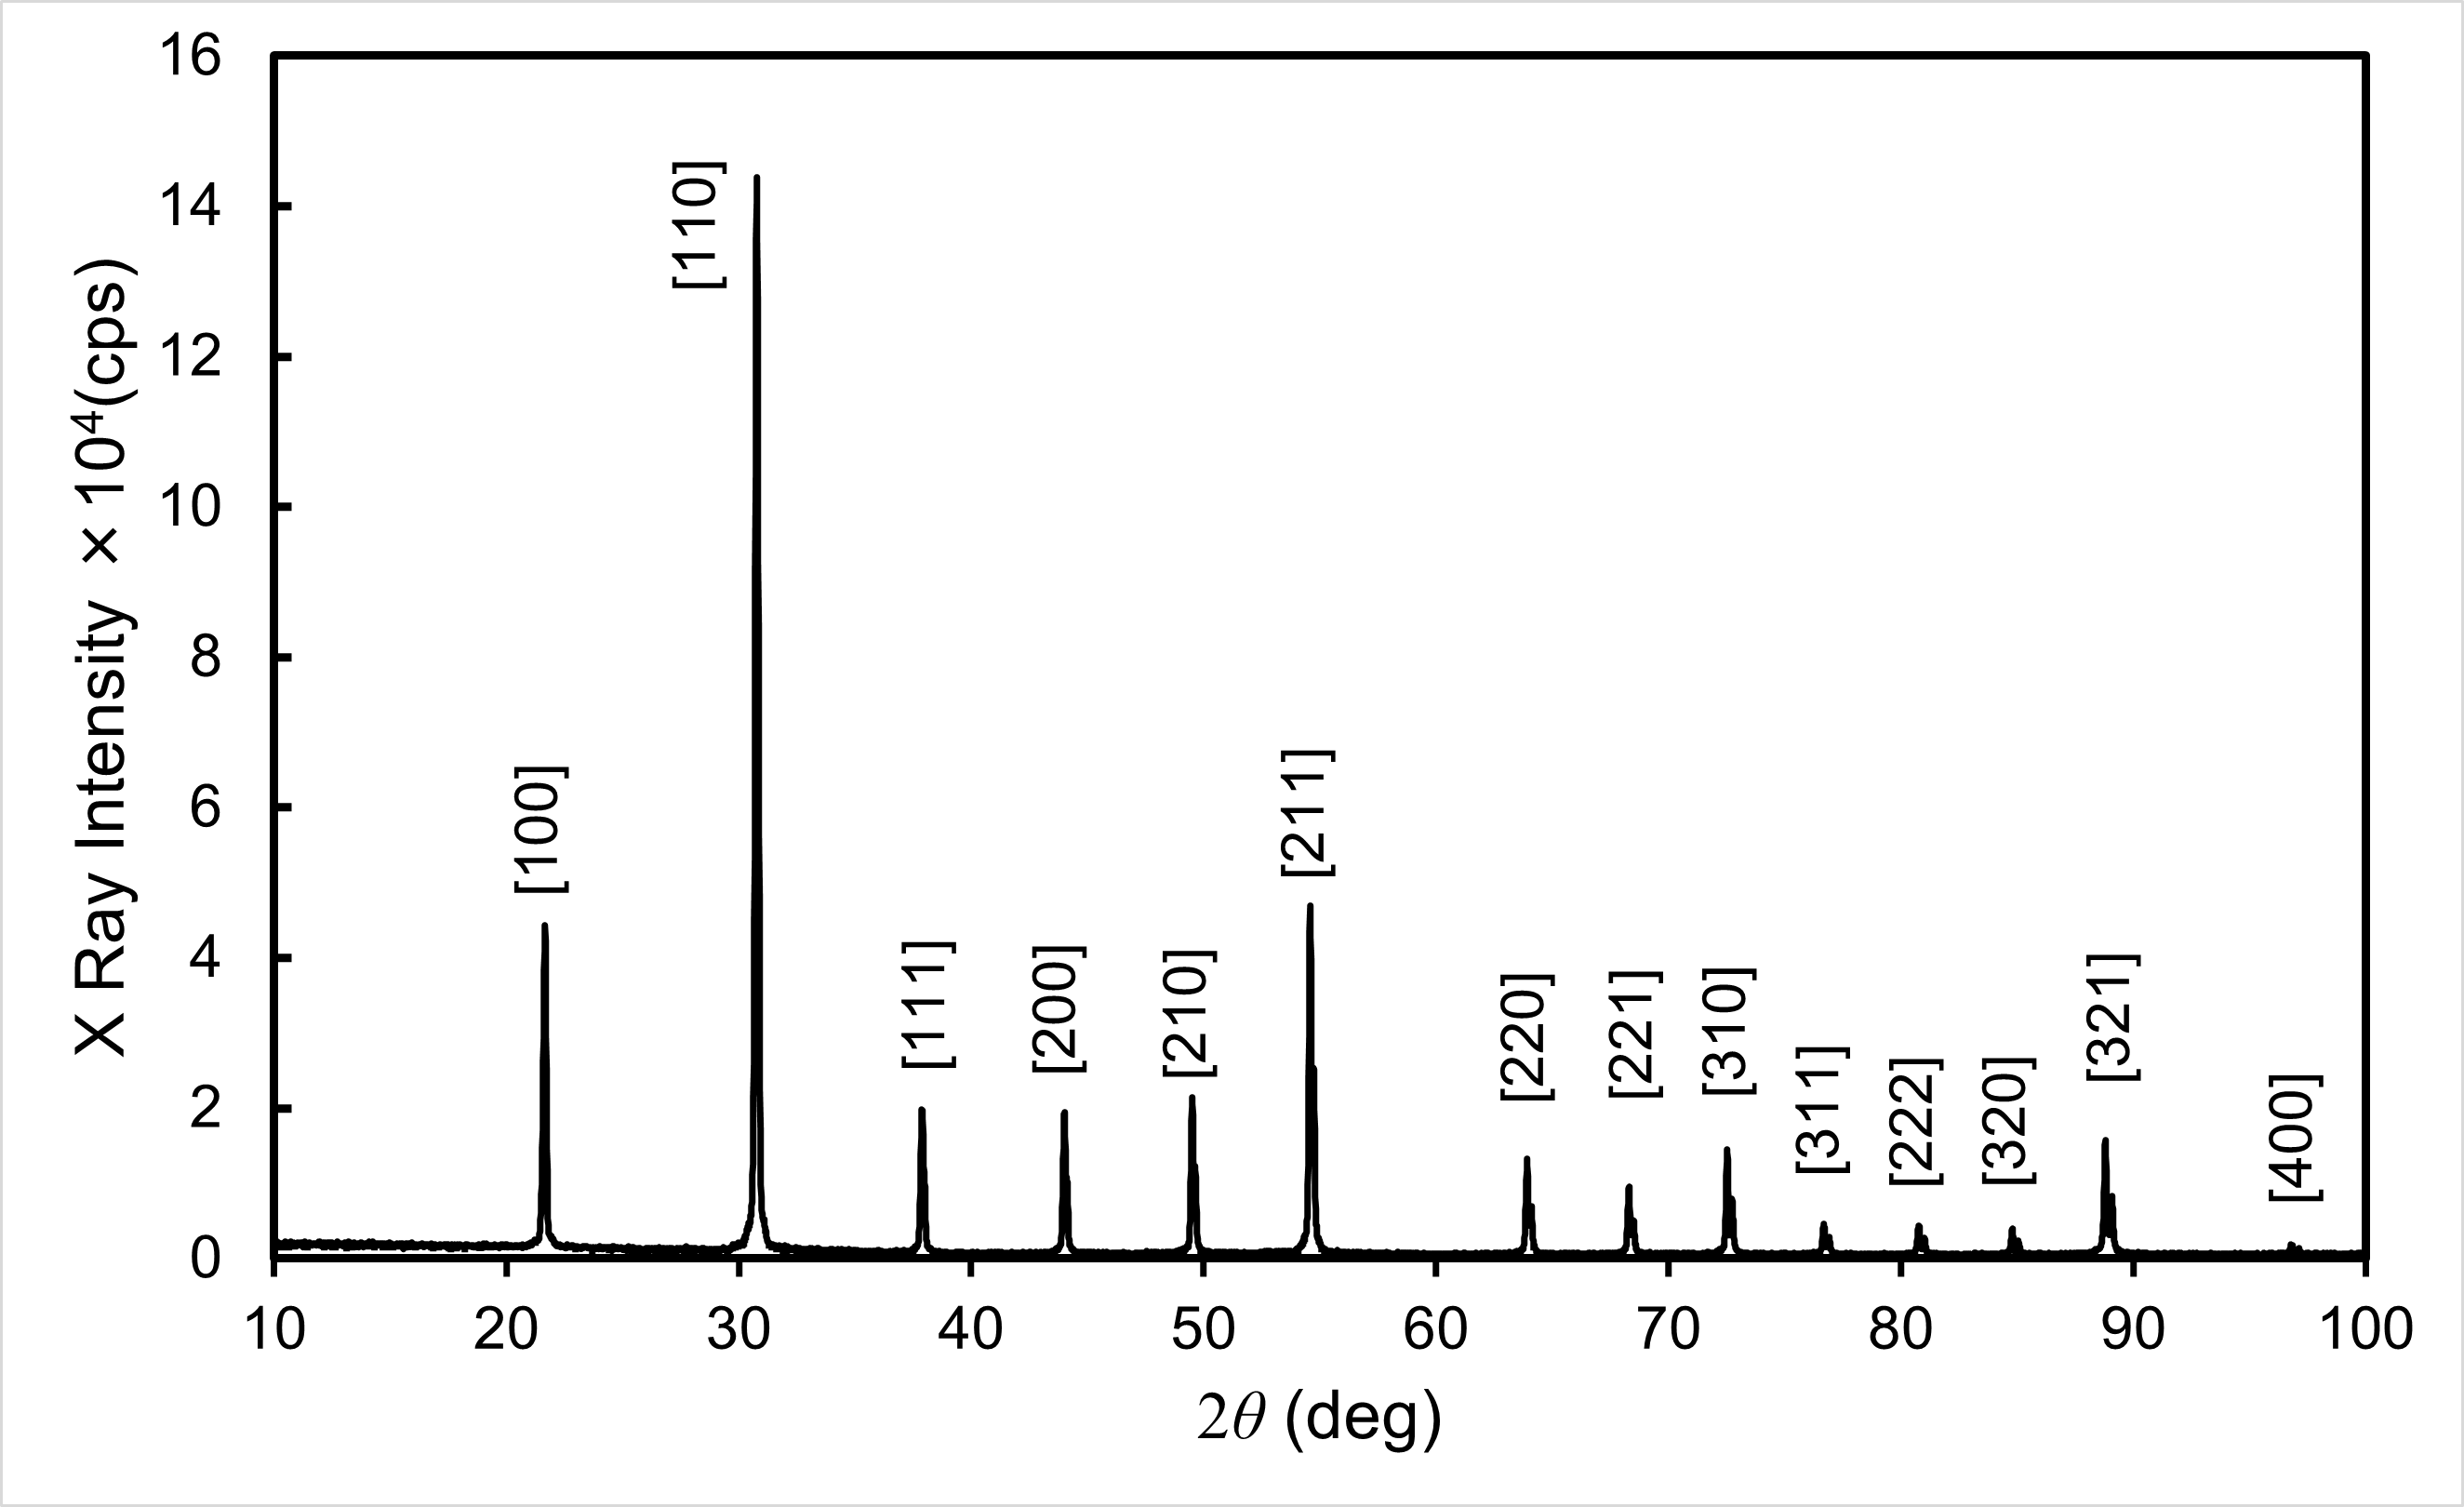
\includegraphics[width=\columnwidth]{/graph/CsCl.png}
% 		\caption{CsCl 粉末の X 線回折強度}
% 		\label{CsCl_XRD}
% 	\end{minipage}
% \end{figure}

\section{課題}
\subsection*{課題1}
以下の 3 組の、結晶構造が同じ、あるいは似た試料の XDR 回折の結果を比較して、違いが出る理由を考察せよ。\\
(i) Fe と CsCl \quad (ii) Cu と Si \quad (iii) NaCl と KCl\\ \\

\subsubsection*{(1)}
しかし散乱強度における結晶構造因子を考えると Fe の場合
\begin{align}
	F = f_{\text{fe}}\qty(1+e^{i\pi(h+k+l)})
\end{align}
なのに対し CsCl は
\begin{align}
	F = f_{\text{Cs}}+f_{\text{Cl}}e^{i\pi(h+k+l)}
\end{align}
となる。CsCl の原子散乱因子は Cs と Cl では違うので、
面指数[hkl] の和が奇数のときであっても消滅則が働かない。
そのため XDR で検出したピークの数は CsCl のほうが多くなる。% 結果のところに貼った図表番号を入れたい。
Fe の強度が弱くなっているのは Fe 結晶構造というよりかはの特性によるものである。
これは考察で言及する。\\ % あとで具体的にな考察の節番号を振りたい

\subsubsection*{(ii)}
Si はこれにさらに面心立方構造を(1/4, 1/4, 1/4)方向にずらした副格子もある。%副格子ってあってる?
そのため結晶構造因子は Cu のものは
\begin{align}
	F = f_{\text{Cu}}\qty(1+e^{i\pi(h+k)}+e^{i\pi(k+l)}+e^{i\pi(l+h)})
\end{align}
であり、Si は
\begin{align}
	F = f_{\text{Si}}\qty(1+e^{\frac{i\pi}{2}(h+k+l)})\qty(1+e^{i\pi(h+k)}+e^{i\pi(k+l)}+e^{i\pi(l+h)})
\end{align}
となる。
これを見ると Si の XDR のピークが消えずに残る条件は、
面心立方の消滅則である面指数 [hkl] のすべての指数の偶奇が一致しているときに加え、
[hkl] の和を4で割ったあまりが2ではないという条件が加わる。
測定できたピークの数としては Si の方が多いが面間隔のことを考えると、
やはり消滅則が多い Si は消滅しているピークがあることがわかる。% 図の参照を加えたい
Cu にはバックグラウンドが多いことは考察で言及する\\ % かもしれない
\subsubsection*{(iii)}
しかし両者を比較すると KCl では消滅しているピークがある。
これは X 線の回折に関わるイオンの散乱因子の違いからくるであると考えられる。
イオン散乱因子は希ガス核と同じだと考えると、
Na は Ne 核、Cl と K は Ar 核になるので結晶構造因子は
NaCl では
\begin{align}
	F = \qty(f_{\text{Ne}}+f_{\text{Ar}}e^{i\pi h})\qty(1+e^{i\pi(h+k)}+e^{i\pi(k+l)}+e^{i\pi(l+h)})
\end{align}
となり、KCl では
\begin{align}
	F = f_{\text{Ar}}\qty(1 + e^{i\pi h})\qty(1+e^{i\pi(h+k)}+e^{i\pi(k+l)}+e^{i\pi(l+h)})
\end{align}
となる。
これより面指数 h が奇数か偶数かという消滅則が KCl には働く。

\subsection*{課題2} 仮にこれらの立方晶の物質が、
何らかの摂動を受けて正方晶になったとする。
このとき、X 線回折パターンにはどのような変化が起こるかを推測せよ。
そして測定した物質の中から1つを例にとり、この推測に沿って具体的に議論せよ。\\

定性的には[111]面のような等方的な面によるピークは変わらず、
[220]のような面指数が異なる面によるピークは 1:2 の強度比で分裂するであろうと考えられる。

面指数[111]はどの指数を c 軸に取ったとしてもその面の形状は変わらない。% 図を描きたい
しかし[220]のときは指数が2の方向を c 軸に取るのと、面指数が0の方向を c 軸に取るのとでは面の形状は変わる。
c 軸の取り方は面指数が 2 の方向を取るのは 2 通り、 0 の方向を取るのは 1 通りであるため、
粉末にしたとき面の向く割合が 1:2 になるため強度のピークは変わる。

まとめると c 軸だけ伸びたとき面指数[hkl]の示す面が変わるかどうかによる。

\subsection*{課題3}
Cu の粉末 X 線回折結果の強度比 \(I^{\text{obs.}}\)と
付録に説明してある式 (S1)を利用して計算した強度比 \(I^{\text{cal.}}\)
を比較し、議論せよ。
ここで強度比は、最も強い回折ピークの強度を 100 として答えよ。

\section{考察}
\subsection{Fe の X 線回折強度について}
a\cite{rikanenpyo}

\subsection{イオン結晶の発光}


\section{結論}

\bibliographystyle{junsrt}
\bibliography{reference}
\section*{付録}

\end{document}